\section{Architettura}\label{architettura}
\subsection{Scopo del Capitolo}
Il seguente capitolo ha lo scopo di fornire le informazioni necessarie allo sviluppatore per potersi interfacciare con il prodotto, in modo tale da rendere più agevole l'ampliamento e la modifica.

\subsection{Visione Generale}\label{archGenerale}
Il prodotto si basa su 3 componenti chiave: 
\begin{itemize}
	\item Il cliente, ovvero il plug-in per \textit{Grafana}; 
	\item Il server, il quale agisce da controller; 
	\item Il database che fornisce il model.
\end{itemize}
Queste tre componenti unite formano il prodotto finale. Esse cambiano messaggi e informazioni una con le altre seguendo un pattern meglio conosciuto come MVC\glossario 

\begin{figure}[H]
	\begin{center}
		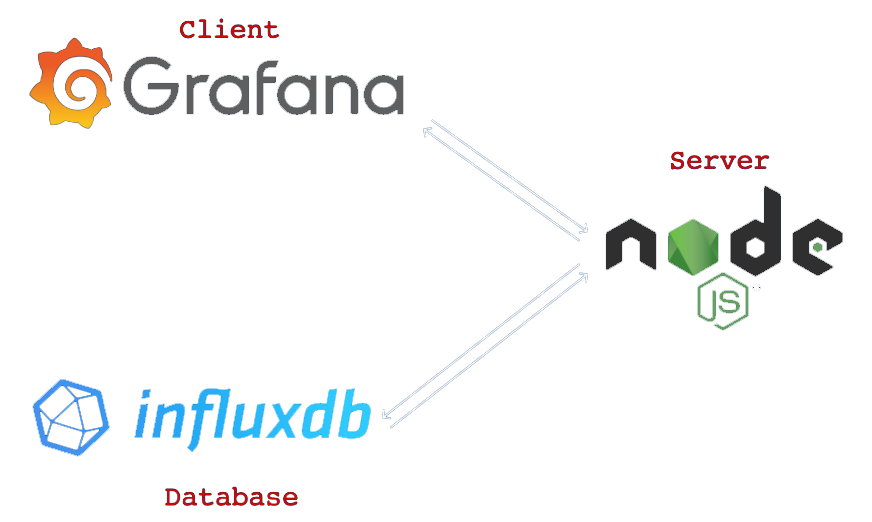
\includegraphics[scale=0.5]{./images/architettura.png} 
	\end{center}
	\caption{Architettura dell'applicativo}
\end{figure}


\subsection{Pannello}\label{archPannello}
Per rendere lo sviluppo più semplice, e garantire la manutenibilità del codice il team ha optato per un approccio modulare. In questo modo, avendo moduli separati con compiti distinti, sarà più semplice modificarne o estenderne il comportamento senza dover necessariamente modificare la base comune.\\
In particolare i moduli separati sono:
\begin{itemize}
	\item \textbf{GBCtrl}: è il modulo principale che utilizza gli altri e svolge le operazioni fondamentali;
	\item \textbf{TemporalPolicyCtrl}: è il modulo che si occupa di gestire ed impostare le politiche temporali all'interno del pannello;
	\item \textbf{ThresholdsCtrl}: è il modulo che si occupa di gestire ed impostare le soglie per il monitoraggio;
	\item \textbf{Parser}: è il modulo che si occupa di controllare e interpretare la rete bayesiana in input, in formato \textit{JSON};
	\item \textbf{ConnectServerProxy}: è il modulo che si occupa di inoltrare le richieste al server preoccupandosi che i dati siano strutturati nel modo corretto e ricevere i dati;
	\item \textbf{ModalCreator}: è il modulo che si occupa di visualizzare le finestre che permettono l'interazione con l'utente;
	\item \textbf{GetAPIGrafana}: è il modulo che si occupa di interagire con le API di \textit{Grafana} per ottenere i dati relativi alle sorgenti dati.
\end{itemize}

\subsubsection{UML - Diagramma dei Package}
\begin{figure}[H]
\begin{center}
	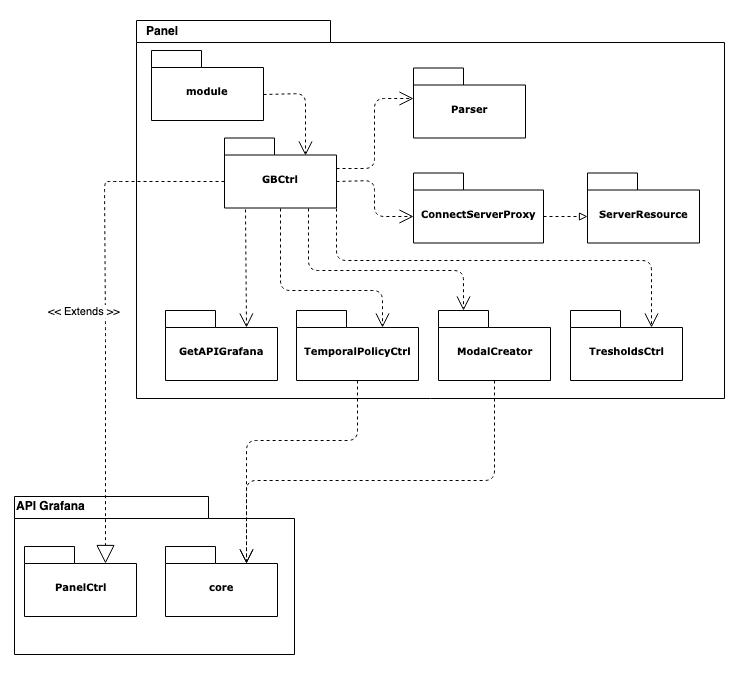
\includegraphics[scale=0.6]{./images/panelPackage.png} 
\end{center}
\caption{Diagramma dei Package del Pannello}
\end{figure}

\begin{landscape}
\subsubsection{UML - Diagramma delle Classi}
\begin{figure}[H]
	\begin{center}
		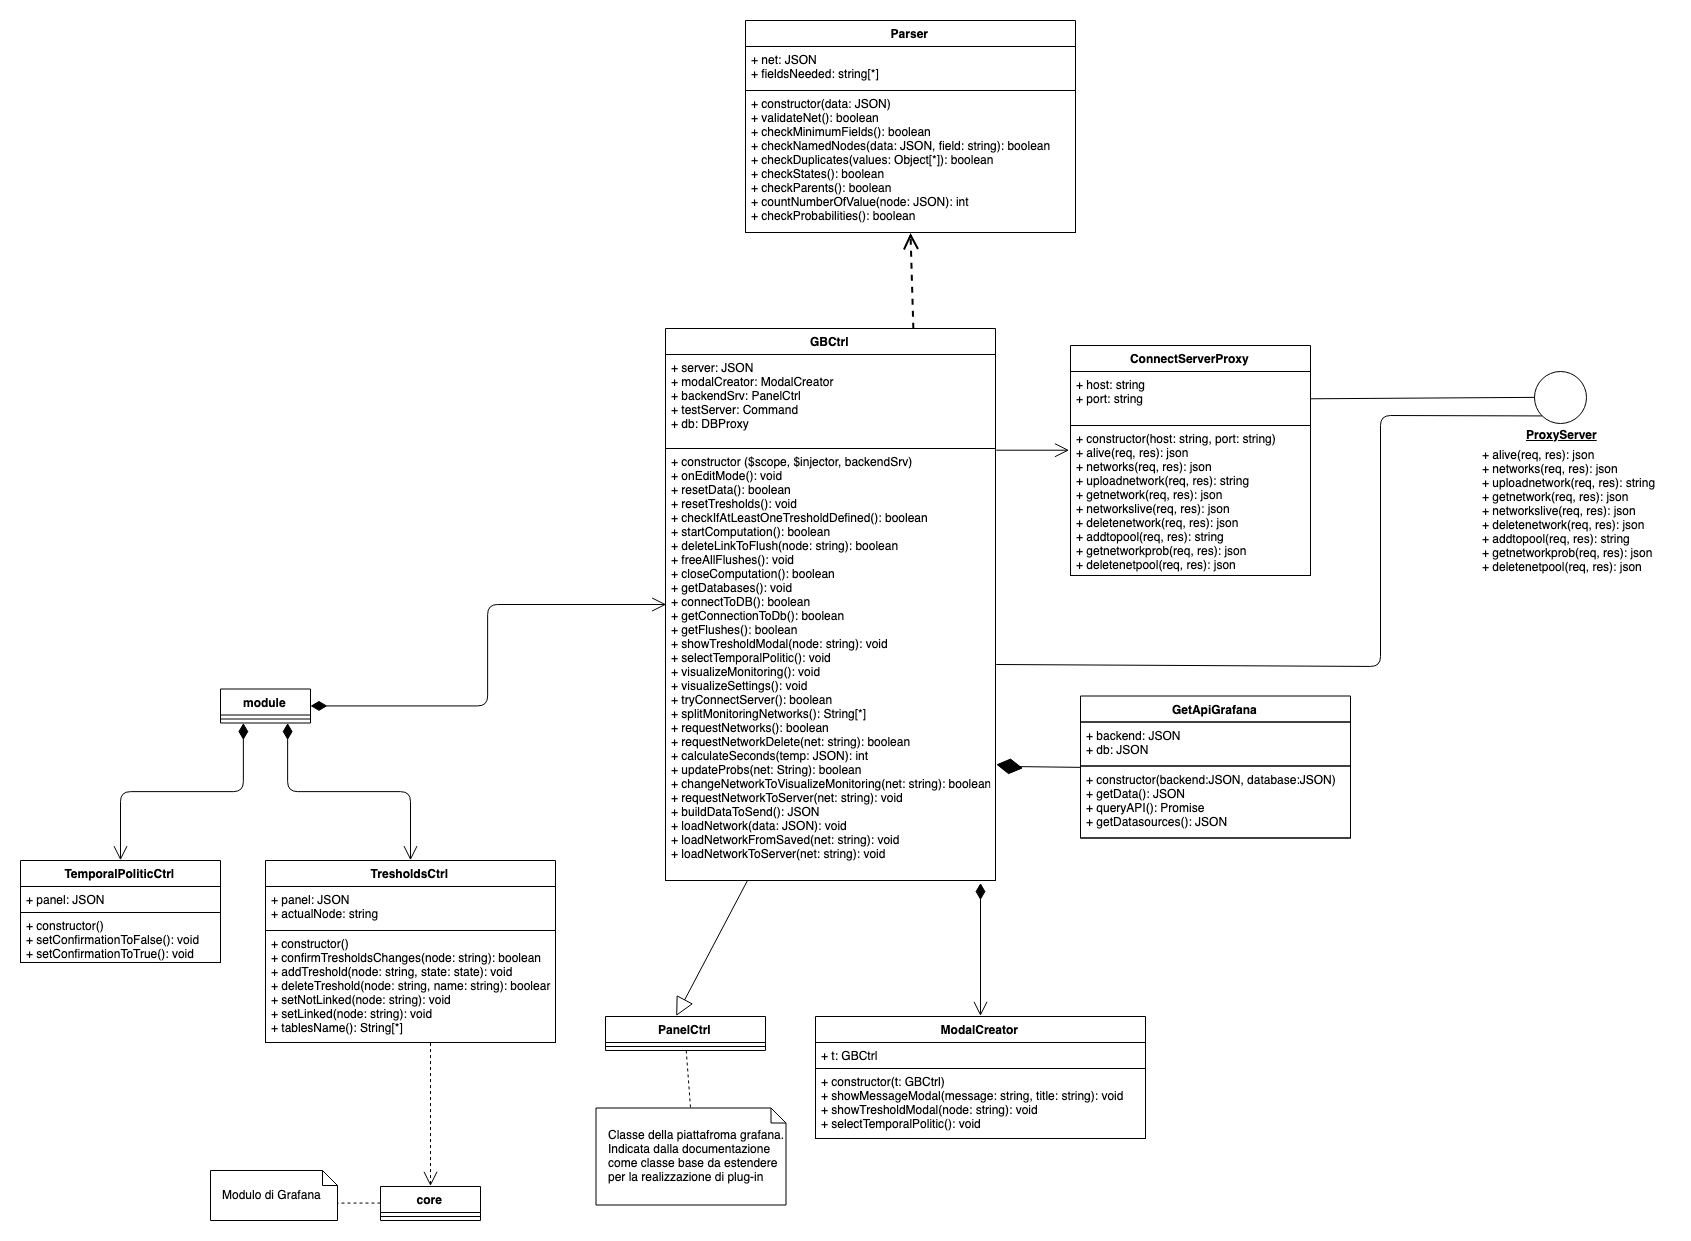
\includegraphics[scale=0.27]{./images/panelClassi.png} 
	\end{center}
	\caption{Diagramma delle Classi del Pannello}
\end{figure}
\end{landscape}


\subsection{Server}\label{archServer}
Per rendere lo sviluppo più semplice, e garantire la manutenibilità del codice il team ha optato per un approccio modulare. In questo modo, avendo moduli separati con compiti distinti, sarà più semplice modificarne o estenderne il comportamento senza dover necessariamente modificare la base comune.\\
In particolare i moduli presenti per quanto riguarda lo sviluppo del server sono:
\begin{itemize}
	\item \textbf{Server}: è il modulo principale che si occupa di comunicare con gli altri, ed esegue le operazioni fondamentali;
	\item \textbf{InfluxDB}: è il modulo che si occupa di adattare la libreria \textit{Influx} e ci fornisce un set di metodi specializzati;
	\item \textbf{Network}: è il modulo che si occupa di adattare la libreria \textit{jsbayes} e costruisce la rete bayesiana da utlizzare;
	\item \textbf{ProxyServer}: è il modulo che si occupa di filtrare, autenticare le richieste verso il server e  protegge lo stesso.
\end{itemize}


\subsubsection{UML - Diagramma dei Package}
\begin{figure}[H]
	\begin{center}
		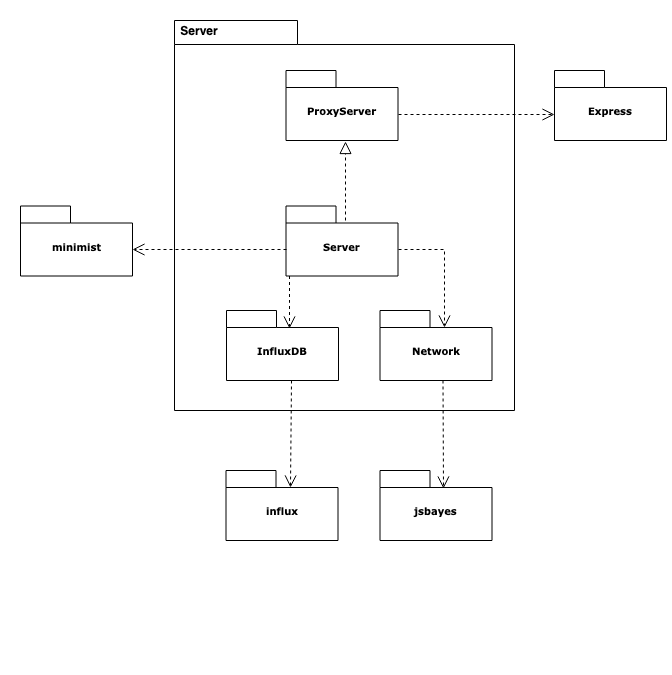
\includegraphics[scale=0.6]{./images/serverPackage.png} 
	\end{center}
	\caption{Diagramma dei Package del Server}
\end{figure}

\begin{landscape}
\subsubsection{UML - Diagramma delle Classi}
\begin{figure}[H]
	\begin{center}
		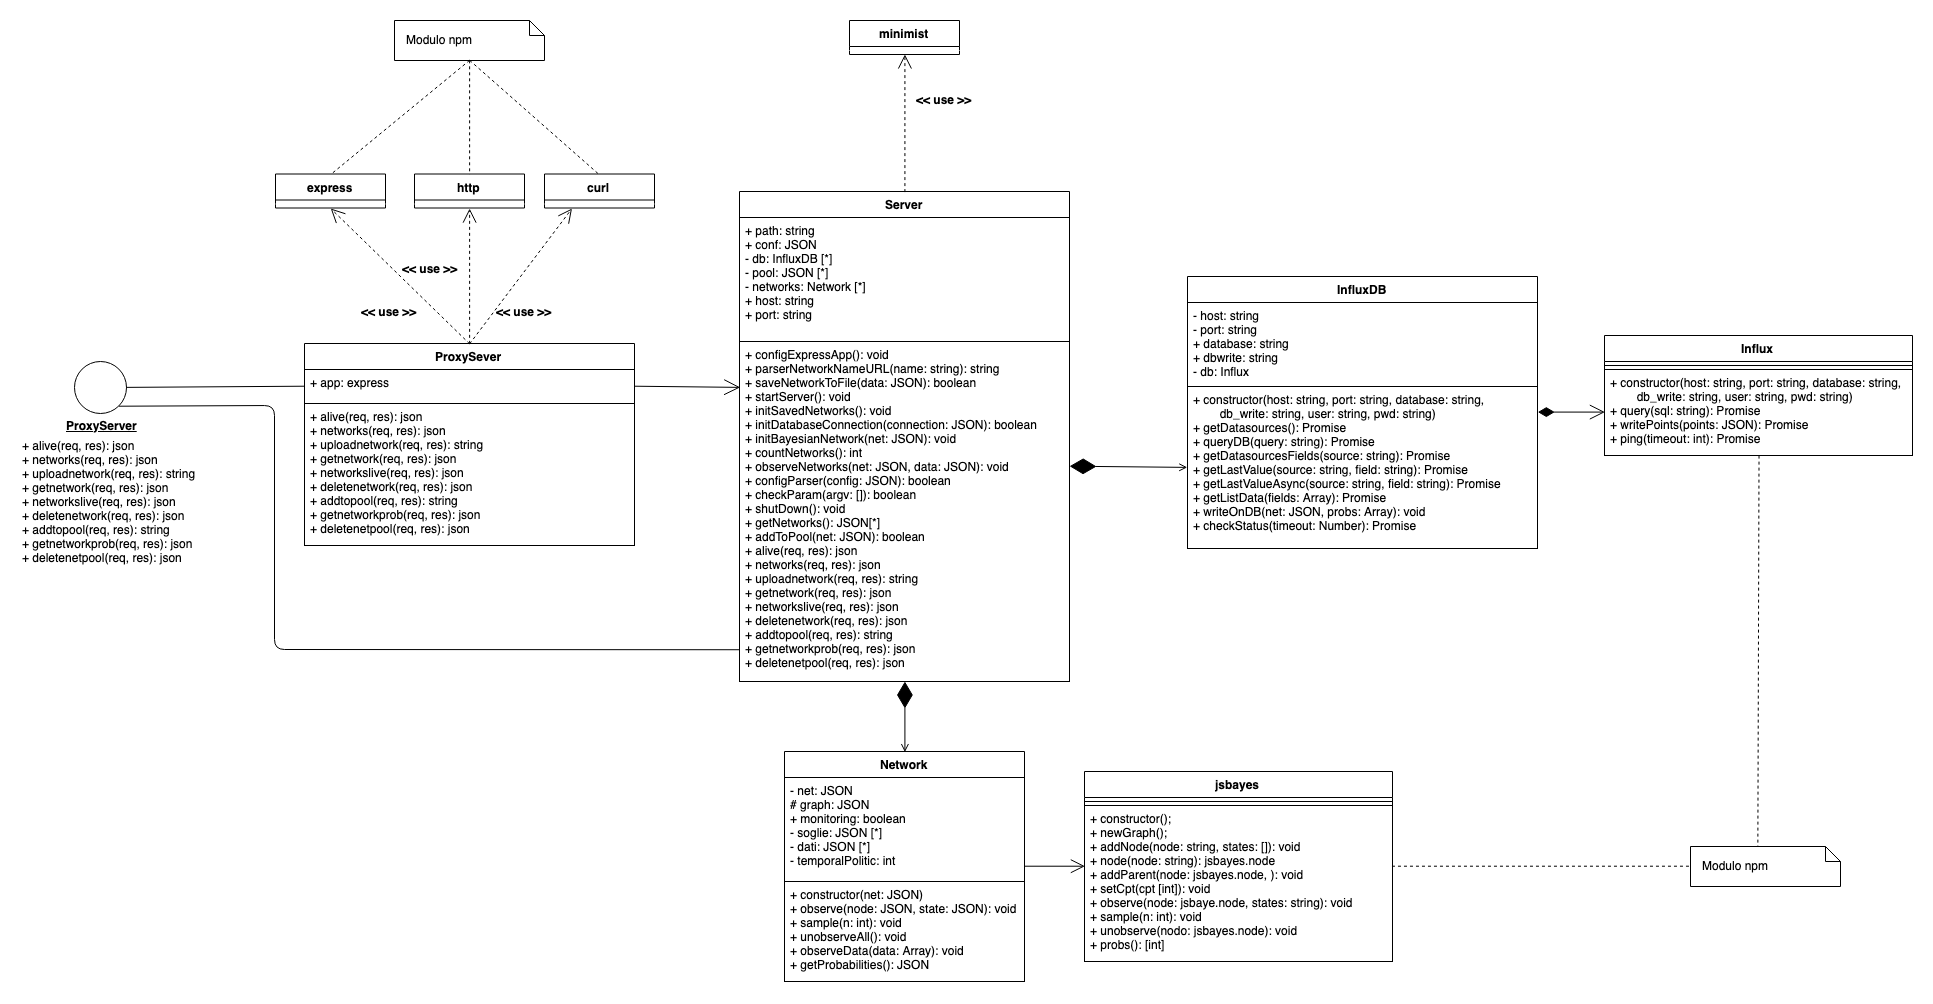
\includegraphics[scale=0.35]{./images/serverClassi.png} 
	\end{center}
	\caption{Diagramma delle Classi del Server}
\end{figure}
\end{landscape}

